\section{Part III - Multivariable control} \label{sec:part3}
%%%% 5.3
The goal with this part of the lab is to control the pitch angle and elevation rate with a multivariable controller. The pitch angle and elevation rate were given from the joystick and were used as reference. 

\subsection{Problem 1}
First task is to calculate \textbf{A} and \textbf{B} from equations \eqref{6a} - \eqref{6c}, for the given state-space model of the form 
\begin{equation*} 
    \boldsymbol{\dot{x} = Ax + Bu}
\end{equation*}
The state vectors and input vectors are given as
\[
    \boldsymbol{x}=\begin{bmatrix}
    \tilde{p}\\
    \dot{\tilde{p}}\\
    \dot{\tilde{e}}
  \end{bmatrix},
\boldsymbol{u}= \begin{bmatrix}
   \tilde{V}_s\\
   \tilde{V}_d
\end{bmatrix}
\]
After some matrix calculation the matrices A and B was found to be
\begin{subequations}
\begin{align}
    \boldsymbol{A} = \begin{bmatrix} \label{A2 Matrix}
    0 & 1 & 0 \\
    0 & 0 & 0 \\
    0 & 0 & 0
    \end{bmatrix}
\\ 
    \boldsymbol{B} = \begin{bmatrix} \label{B2 Matrix}
    0 & 0 \\
    0 & K_1 \\
    K_2 & 0 
    \end{bmatrix}
    \end{align}
    \end{subequations}
Where $K_1$ is \eqref{eq:K_1} and $K_2$ is \eqref{eq:K_2}. 

\subsection{Problem 2}
A PD controller was used to track the reference \textbf{r} =$ [\tilde{p}_c , \dot{\tilde{e}}_c]^T$. The controller was transformed to a linear quadratic regulator (LQR). The matrix \textbf{K} corresponds to the LQR for control input $\textbf{u} = -\textbf{Kx}$. This optimized the cost function.
\begin{equation*}
        J = \int_{0}^{\infty}(\boldsymbol{x}^T(t) \boldsymbol{Qx}(t) +\boldsymbol{u}^T(t)\boldsymbol{Ru}(t))dt
\end{equation*}
The task now was to examine the controllability of the system. If a system is controllable, (ie. the controllability matrix \textbf{C}, has full row rank), then the eigenvalues of the system can be places exactly as desired. The motivation for choosing the eigenvalues is that they are also the poles of the system. The poles affects the system in multiple ways like stability, convergence rate and noise immunity. 
\newline
The stability matrix was calculated with the following formula.
\begin{subequations}
\begin{align*}
\textbf{C} = \begin{bmatrix}
    \boldsymbol{B} &
    \boldsymbol{AB} &
    . &
    .&
    \boldsymbol{A^nB}
    \end{bmatrix}
\end{align*}
\end{subequations}
\begin{equation}
\textbf{C}= \begin{bmatrix}\label{cont matrix}
    0 & 0 & 0 & K_1 & 0 & 0\\
    0 & K_1 & 0 & 0 & 0 & 0\\
    K_2 & 0 & 0 & 0 & 0 & 0\\
\end{bmatrix}
\end{equation}
The system was controllable because the controllability matrix \eqref{cont matrix} had full rank. Ref \cite{syllabus} theorem 6.01. The controller was given on the form 
\begin{equation}
    \boldsymbol{u = Pr -Kx}
\end{equation}
Where \textbf{K} was found with the MATLAB command \textbf{K} = \texttt{lqr}(\textbf{A, B, Q, R}), and P was calculated as $\boldsymbol{P} =\boldsymbol{[C[BK -A]}^{-1}\boldsymbol{ B]}^{-1}$.
The matrix \textbf{C} was found from the following equation
\begin{equation}\label{eq:output}
    \boldsymbol{y = Cx}
\end{equation}
\[
    \begin{bmatrix}
    \tilde{p}\\
    \dot{\tilde{e}}
    \end{bmatrix}
=
    \begin{bmatrix}
    1 & 0 & 0 \\
    0 & 0 & 1
    \end{bmatrix}
    \begin{bmatrix}
    \tilde{p}\\
    \dot{\tilde{p}}\\
    \dot{\tilde{e}}
    \end{bmatrix}
\]
The MATLAB code can be seen in Appendix \ref{sec:matlab_code}.
The system was implemented in Simulink (see \cref{sim:u=p3p2}). For tuning the LQR the matrices \textbf{Q} and \textbf{R} were picked out to be diagonal. \textbf{R} was chosen to be 1 at the diagonal because this made it easier to find the values of \textbf{Q}. For \textbf{Q}, it was desirable that the system be more "concerned" with the error of $\tilde{p}$ and $\dot{\tilde{e}}$, which are the reference values. Different values of \textbf{Q} were tested, and the reference-signal value was plotted with the output-signal.
\begin{figure}[H]
\graphicspath{ {Part3_pictures/}}
\begin{subfigure}{0.5\textwidth}
    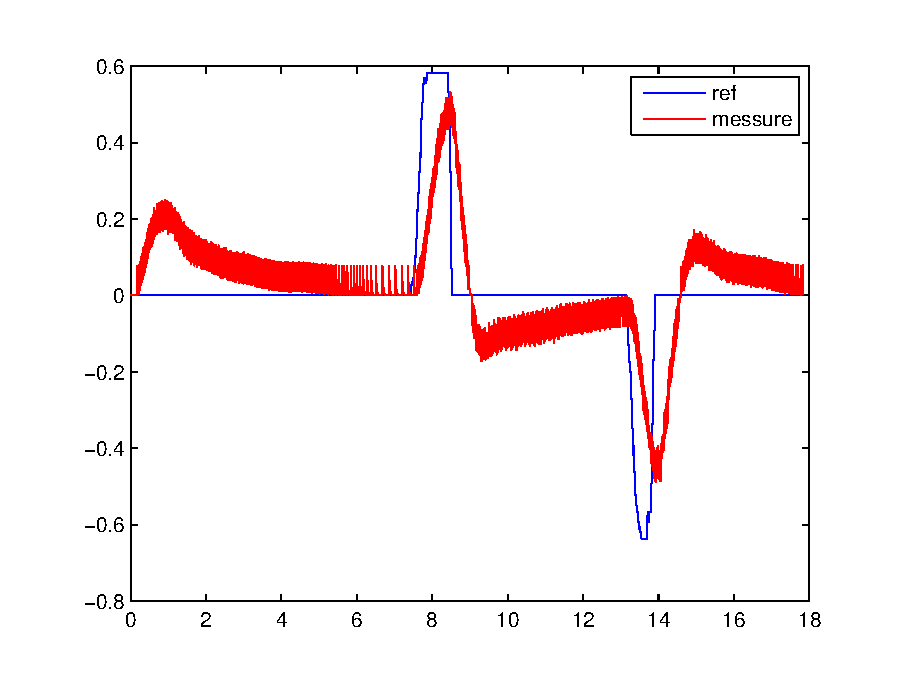
\includegraphics[width=0.9\linewidth]{Part3_pictures/p3p2/Q5elevation.eps} 
    \caption{Elevation rate}
    \label{p3p2Q4e}
\end{subfigure}
\begin{subfigure}{0.5\textwidth}
    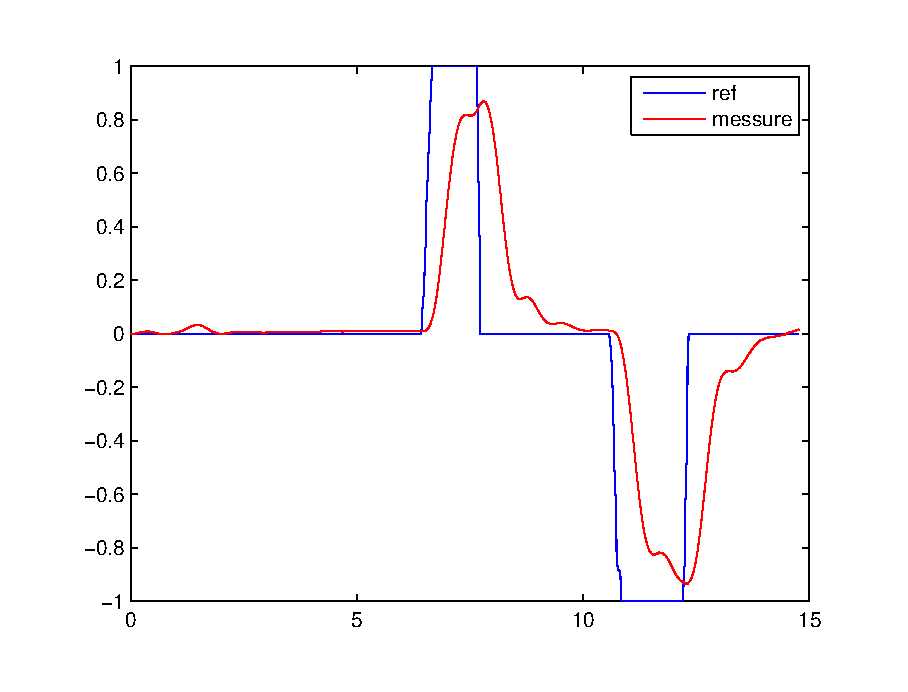
\includegraphics[width=0.9\linewidth]{Part3_pictures/p3p2/Q5pitch.eps}
    \caption{Pitch angle}
    \label{p3p2Q4p}
\end{subfigure}
\caption{Plot with Q = [150 10 250]}
\label{p3p2Q4}
\end{figure}
The goal was a fast and accurate helicopter. With \textbf{Q} = [150 10 250], the helicopter was fast for the elevation angle but did get some overshoot. The pitch angle was found accurate and sufficiently fast. This result caused the helicopter to fall in height slowly when the joystick was released and the reason for that is that the LQR is a PD controller, which will not remove stationary deviation.
\newline\newline
The signal for measured pitch angle looked smooth and with little noise, but the measured signal for the elevation rate looked very noisy. This is because the signals measured are discrete, and since the system doesn't have a way to measure the travel, elevation or pitch rate, they have to be calculated. This is done by derivation of the angles, which are discrete signals interpreted as impulses. Derivation of impulses gives values to infinity, which will make the signal look noisy while in fact it's just a calculation error.

\subsection{Problem 3}

The helicopter was then controlled by a PI regulator with an LQR. To implement the integral effect, two differential equations were given by 
\begin{subequations}
    \begin{gather}
       \dot{\gamma}= \tilde{p} - \tilde{p}_c\\
       \dot{\zeta} = \dot{\tilde{e}} - \dot{\tilde{e}}_c
    \end{gather}
\end{subequations}
The new state vector and the input vector then became 
\[
    \boldsymbol{x}=\begin{bmatrix}
    \tilde{p}\\
    \dot{\tilde{p}}\\
    \dot{\tilde{e}}\\
    \dot{\gamma}\\
    \dot{\zeta}
  \end{bmatrix},
\boldsymbol{u}= \begin{bmatrix}
   \tilde{V}_s\\
   \tilde{V}_d
\end{bmatrix}
\]
The system was then rewritten to the following state-space model
\begin{equation*}
    \boldsymbol{\dot{x} = Ax +Bu + Fr}
\end{equation*}

\[
\begin{bmatrix}
    \dot{\tilde p} \\
    \ddot{\tilde{p}}\\
    \ddot{\tilde e}\\ 
    \dot{\gamma}\\
    \dot{\zeta}
\end{bmatrix}
=
\begin{bmatrix}
    0 & 1  & 0 & 0 & 0\\
    0 & 0  & 0 & 0 & 0\\
    0 & 0  & 0 & 0 & 0\\
    1 & 0  & 0 & 0 & 0\\
    0 & 0  & 1 & 0 & 0
\end{bmatrix}
\begin{bmatrix}
    \tilde {p} \\
    \dot{\tilde{p}}\\
    \tilde{\lambda}\\
    \gamma\\
    \zeta
 \end{bmatrix}
 + 
 \begin{bmatrix}
    0 & 0 \\
    0 & K_1 \\
    K_2 & 0 \\
    0 & 0\\ 
    0 & 0
\end{bmatrix}
\begin{bmatrix}
    \tilde{V_s}\\
    \tilde{V_d}\\ 
\end{bmatrix}
+
 \begin{bmatrix}
    0 & 0 \\
    0 & 0 \\
    0 & 0 \\
    -1 & 0\\ 
    0 & -1
\end{bmatrix}
\begin{bmatrix}
    \tilde{p}_c\\
    \dot{\tilde{e}}_c
\end{bmatrix}
\]
The \textbf{Q} will be a 5x5 matrix. The output matrix \textbf{y} is given by 
\[
    \begin{bmatrix}
    \tilde{p}\\
    \dot{\tilde{e}}
    \end{bmatrix}
=
    \begin{bmatrix}
    1 & 0 & 0 & 0 & 0 \\
    0 & 0 & 1 & 0 & 0
    \end{bmatrix}
 \begin{bmatrix}
    \tilde {p} \\
    \dot{\tilde{p}}\\
    \tilde{\lambda}\\
    \gamma\\
    \zeta
 \end{bmatrix}
\]
Appendix \ref{sec:matlab_code}\ref{lst:p3p3} shows the implementation of the calculation in MATLAB. The different plots are for different values for \textbf{Q}. It was observed that when the system had to large cost on a signal, the helicopter started to vibrate. This was because the system tried to hard to regulate toward the small errors from the reference and the measured signal. After trying out different values for \textbf{Q} the best result found is showed in \cref{p3p351}.

\begin{figure}[H]
\graphicspath{ {Part3_pictures/}}
\begin{subfigure}{0.5\textwidth}
    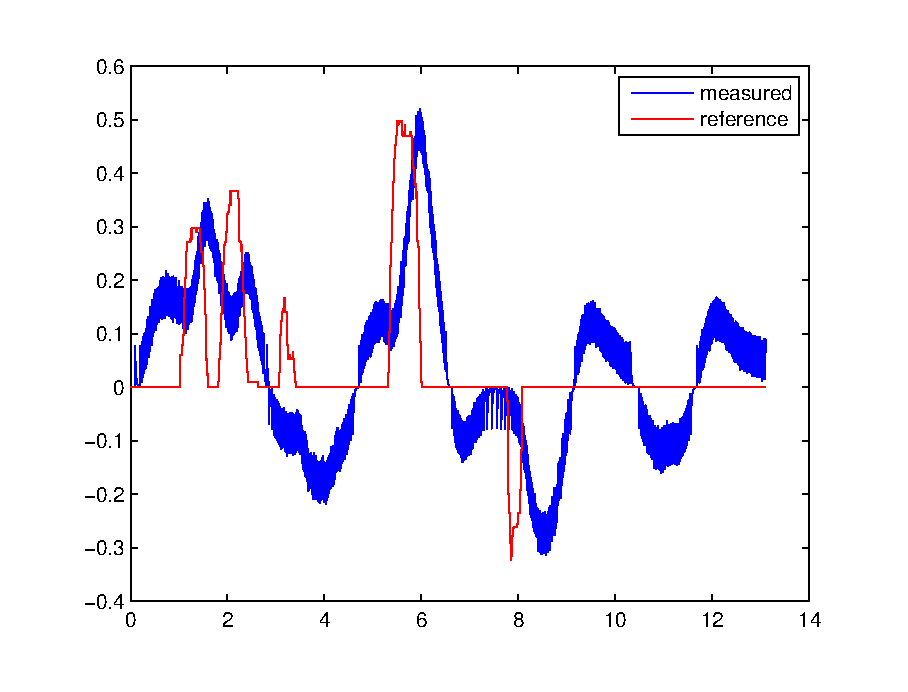
\includegraphics[width=0.9\linewidth]{Part3_pictures/p3p3/Q5elevation.eps} 
    \caption{Elevation rate}
    \label{p3p3Q5e}
\end{subfigure}
\begin{subfigure}{0.5\textwidth}
    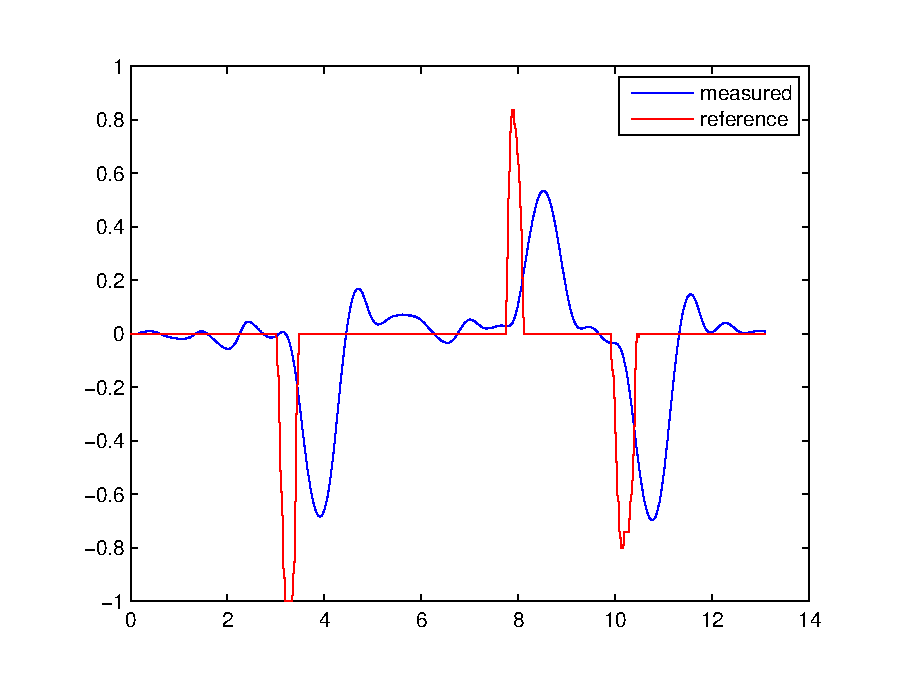
\includegraphics[width=0.9\linewidth]{Part3_pictures/p3p3/Q5pitch.eps}
    \caption{Pitch angle}
    \label{p3p2Q5p}
\end{subfigure}
\caption{Plott with Q =[150 10 250 25 140]}
\label{p3p351}
\end{figure}

By choosing the \textbf{Q} = [150 10 250 25 140], the overshoot was not as big as in the PD controller. The PID was as fast as the PD controller, and the system could now follow the pitch angle reference better. The biggest difference from the two controllers was the plot of the elevation rate. The PID regulator was also able to hold the helicopter to the equilibrium point for the elevation angle, after released the joystick. This was expected because a PID regulator removes the stationary error. A different observation was that with PID the helicopter did not reach the equilibrium point for the elevation angle at the start. This because the actuating signal would give a ramp signal opposing to the integral effect. With higher value for the integral effect, the faster the helicopter would stop the elevation at the powering of the helicopter.  